\documentclass[12pt, openright, oneside, a4paper, english]{abntex2}



% ---
% Pacotes básicos 
% ---
\usepackage{lmodern}			% Usa a fonte Latin Modern			
\usepackage[T1]{fontenc}		% Selecao de codigos de fonte.
\usepackage[utf8]{inputenc}		% Codificacao do documento (conversão automática dos acentos)
\usepackage{lastpage}			% Usado pela Ficha catalográfica
\usepackage{indentfirst}		% Indenta o primeiro parágrafo de cada seção.
\usepackage{color}				% Controle das cores
\usepackage{graphicx}			% Inclusão de gráficos
\usepackage{microtype} 			% para melhorias de justificação
\usepackage{amsthm}
\usepackage{amsmath}
\usepackage{mathtools}
\usepackage{amsfonts}
\usepackage{amssymb}
%\usepackage{mathtools}
\usepackage{caption}
\usepackage{subcaption}
\usepackage{tabularx}
\usepackage{csquotes}
\usepackage{makecell}

% \usepackage{subfigure}

%\usepackage{kbordermatrix}
\usepackage{amsmath}

% \usepackage[portuguese,ruled,lined,linesnumbered]{algorithm2e}
\usepackage[ruled,lined,linesnumbered]{algorithm2e}
% \renewcommand{\algorithmcfname}{Algorithm}

\usepackage{multirow}

\usepackage[brazil]{babel}
\addto\captionsbrazil{%
\def\bibname{References}%
\renewcommand{\figurename}{Figure}
\renewcommand{\tablename}{Table}
\renewcommand{\listfigurename}{List of Figures}
\renewcommand{\listtablename}{List of Tables}
\renewcommand{\contentsname}{Contents}
\renewcommand\chaptername{Chapter}
}

\selectlanguage{english}


% ---
		
% ---
% Pacotes adicionais, usados apenas no âmbito do Modelo Canônico do abnteX2
% ---
\usepackage{lipsum}				% para geração de dummy text
% ---

% ---
% Pacotes de citações
% ---
%\usepackage{backref}	 % Paginas com as citações na bibl
%\usepackage[alf,abnt-and-type=&]{abntex2cite}	% Citações padrão ABNT
\usepackage[alf]{abntex2cite}	% Citações padrão ABNT


%\newtheorem{mydef}{Definição}[chapter]

%\usepackage{natbib}

% --- 
% CONFIGURAÇÕES DE PACOTES
% --- 

% ---
% Configurações do pacote backref
% Usado sem a opção hyperpageref de backref
%\renewcommand{\backrefpagesname}{Citado na(s) página(s):~}
% Texto padrão antes do número das páginas
%\renewcommand{\backref}{}
% Define os textos da citação
%\renewcommand*{\backrefalt}[4]{
%	\ifcase #1 %
%		Nenhuma citação no texto.%
%	\or
%		Citado na página #2.%
%	\else
%		Citado #1 vezes nas páginas #2.%
%	\fi}%
% ---
\newtheorem{name}{Printed output}

\selectlanguage{english}
\renewcommand{\orientadorname}{Supervisor}







% ---
% Informações de dados para CAPA e FOLHA DE ROSTO
% ---
\titulo{Impacto da competição no spread bancário}
\autor{Henrique de Souza Passos}
\local{Brasilia}
\data{2025}
\orientador{Gandalf, the White}

\instituicao{%
 University of Brasilia
  \par
 Graduate Program in Economics }
\tipotrabalho{Master's Thesis}
% O preambulo deve conter o tipo do trabalho, o objetivo, 
% o nome da instituição e a área de concentração 
\preambulo{Doctoral Thesis presented to the Graduate Program in Economics of the University of Brasilia as a partial requirement to obtain the degree of Masters in Economics}
% ---


% ---
% Configurações de aparência do PDF final

% alterando o aspecto da cor azul
\definecolor{blue}{RGB}{41,5,195}

% informações do PDF
\makeatletter
\hypersetup{
     	%pagebackref=true,
		pdftitle={\@title}, 
		pdfauthor={\@author},
    	pdfsubject={\imprimirpreambulo},
	    pdfcreator={LaTeX with abnTeX2},
		pdfkeywords={abnt}{latex}{abntex}{abntex2}{trabalho acadêmico}, 
		colorlinks=true,       		% false: boxed links; true: colored links
    	linkcolor=blue,          	% color of internal links
    	citecolor=blue,        		% color of links to bibliography
    	filecolor=magenta,      		% color of file links
		urlcolor=blue,
		bookmarksdepth=4
}
\makeatother

% O tamanho do parágrafo é dado por:
\setlength{\parindent}{1.3cm}

% Controle do espaçamento entre um parágrafo e outro:
\setlength{\parskip}{0.2cm}  % tente também \onelineskip

% ---
% compila o indice
% ---
\makeindex

% ----
\begin{document}

% Retira espaço extra obsoleto entre as frases.
\frenchspacing 

% ----------------------------------------------------------
% ELEMENTOS PRÉ-TEXTUAIS
% ----------------------------------------------------------
\pretextual

% ---
% Capa
% ---
\imprimircapa
% ---
\cleardoublepage

% ---
% Folha de rosto
% (o * indica que haverá a ficha bibliográfica)
% ---
\imprimirfolhaderosto
% ---

% ---
% Inserir a ficha bibliografica
% ---
% \begin{fichacatalografica}
% 	\begin{figure}
% 	 \includegraphics[scale=0.9]{ficha2.pdf}
% 	\end{figure}
% \end{fichacatalografica}


% \begin{folhadeaprovacao}
%     \begin{figure}
%      \includegraphics[bb=110 0 0 750]{aprov.pdf}
%     \end{figure}
% \end{folhadeaprovacao}


% ---
% Declaração de autoria
% ---
\newpage
\begin{center}
{\ABNTEXchapterfont\Large\textsc{Statement of Authorship}}
\end{center}

\vspace*{1cm}

I hereby declare that the thesis submitted is my own work. All direct or indirect
sources used are acknowledged as references. I further declare that I have not submitted
this thesis at any other institution in order to obtain a degree. \\

% ---


\newpage
% ---
% Dedicatória
% ---
\begin{dedicatoria}
  \vspace*{\fill}
  \centering
  \noindent
  \textit{ To my friends and family. I am nothing without them.} \vspace*{\fill}
\end{dedicatoria}
% ---



% ---
% Agradecimentos
% ---
\begin{agradecimentos}

I would like to thank all people from The Shire, in particular, my beloved nephew Frodo.

\end{agradecimentos}
% ---

\newpage
% ---
% Epígrafe
% ---
\begin{epigrafe}
    \vspace*{\fill}
	
	    \noindent
		\textit{"One Ring to rule them all, One Ring to find them, One Ring to bring them all and in the darkness bind them.."}
		
		\begin{flushright}
		J. R. R. Tolkien
		\end{flushright}
\end{epigrafe}


% ---
\newpage

 

 

% resumo em português
\setlength{\absparsep}{18pt} % ajusta o espaçamento dos parágrafos do resumo
\begin{resumo}[Abstract]
 \begin{otherlanguage*}{english}


It began with the forging of the Great Rings. Three were given to the Elves, immortal, wisest and fairest of all beings. Seven to the Dwarf-Lords, great miners and craftsmen of the mountain halls. And nine, nine rings were gifted to the race of Men, who above all else desire power. For within these rings was bound the strength and the will to govern each race. But they were all of them deceived, for another ring was made. Deep in the land of Mordor, in the Fires of Mount Doom, the Dark Lord Sauron forged a master ring, and into this ring he poured his cruelty, his malice and his will to dominate all life.


\textbf{Keywords:} Invisibility, Sorcery, Ring

\end{otherlanguage*}
\end{resumo}

\newpage


% ---
% inserir lista de ilustrações
% ---
\pdfbookmark[0]{\listfigurename}{lof}
\listoffigures*
\cleardoublepage
% ---

% ---
% inserir lista de tabelas
% ---
\pdfbookmark[0]{\listtablename}{lot}
\listoftables*
\cleardoublepage
% ---
%\begin{siglas}
  %\item[MSE] Erro médio quadrático
  %\item[FLR] Relacionamento Lógico Fuzzy
%\end{siglas}

% ---
% inserir o sumario
% ---
\pdfbookmark[0]{\contentsname}{toc}
\tableofcontents*
\cleardoublepage
% ---

% ----------------------------------------------------------
% ELEMENTOS TEXTUAIS
% ----------------------------------------------------------
\textual

% ----------------------------------------------------------
% Introdução (exemplo de capítulo sem numeração, mas presente no Sumário)
% ----------------------------------------------------------
\chapter{Introduction}
One ring to rule them all -- see the ring in Figure \ref{fig:ring}

One by one, the free lands of Middle-Earth fell to the power of the Ring, but there were some who resisted. A last alliance of men and elves marched against the armies of Mordor, and on the very slopes of Mount Doom, they fought for the freedom of Middle-Earth. Victory was near, but the power of the ring could not be undone. It was in this moment, when all hope had faded, that Isildur, son of the king, took up his father’s sword.


\begin{figure}
    \centering
    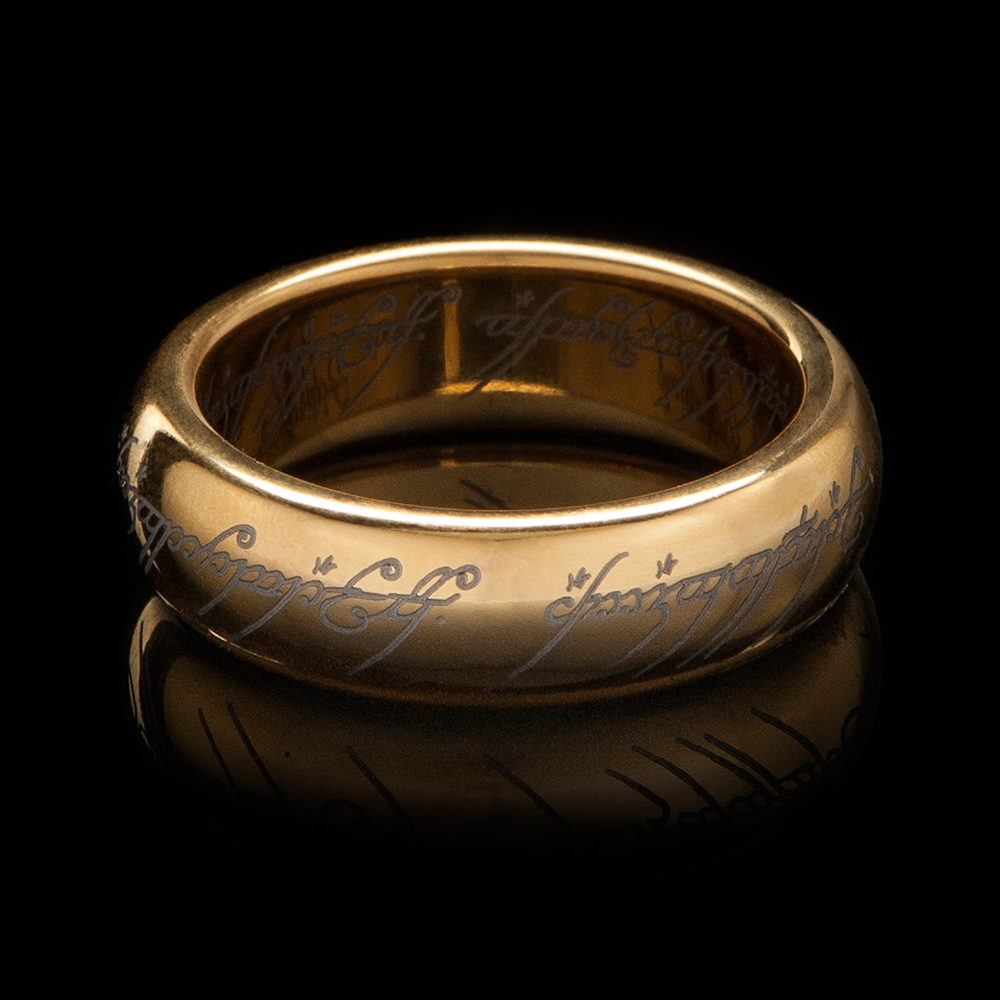
\includegraphics[width=0.5\textwidth]{src/imgs/ring.jpg}
    \caption{An illustration of the powerful ring}
    \label{fig:ring}
\end{figure}


Sauron, enemy of the free peoples of Middle-Earth, was defeated. The Ring passed to Isildur, who had this one chance to destroy evil forever, but the hearts of men are easily corrupted. And the ring of power has a will of its own. It betrayed Isildur, to his death.

And some things that should not have been forgotten were lost. History became legend. Legend became myth. And for two and a half thousand years, the ring passed out of all knowledge. Until, when chance came, it ensnared another bearer \cite{tolkien2012fellowship}.

It came to the creature Gollum, who took it deep into the tunnels of the Misty Mountains. And there it consumed him. The ring gave to Gollum unnatural long life. For five hundred years it poisoned his mind, and in the gloom of Gollum’s cave, it waited. Darkness crept back into the forests of the world. Rumor grew of a shadow in the East, whispers of a nameless fear, and the Ring of Power perceived its time had come. It abandoned Gollum, but then something happened that the Ring did not intend. It was picked up by the most unlikely creature imaginable: a hobbit, Bilbo Baggins, of the Shire.

For the time will soon come when hobbits will shape the fortunes of all.

\chapter{Raug}
At its head there rode a tall and evil shape, mounted upon a black horse, if horse it was; for it was huge and hideous, and its face was a frightful mask, more like a skull that a living head, and in the sockets of its eyes and in its nostrils there burned a flame. The rider was robed all in black, and black was his lofty helm; yet this was no Ringwraith but a living man.

The lieutenant of the Tower of Barad-dúr he was, and his name is remembered in no tale; for he himself had forgotten it, and he said: 'I am the Mouth of Sauron.' But it is told that he was a renegade, who came of the race of those that are named the Black Númenoreans



% ----------------------------------------------------------
% Referências bibliográficas
% ----------------------------------------------------------
\citeoption{abnt-etal-list=5}
\bibliographystyle{abntex2-cite-min}
\bibliography{references}



% ----------------------------------------------------------
% Glossário
% ----------------------------------------------------------
%
% Consulte o manual da classe abntex2 para orientações sobre o glossário.
%
%\glossary

% ----------------------------------------------------------
% Apêndices
% ----------------------------------------------------------

% ---
% Inicia os apêndices
% ---
\begin{apendicesenv}

% Imprime uma página indicando o início dos apêndices
%\partapendices

% ----------------------------------------------------------
\chapter{People who have worn the ring}
% ----------------------------------------------------------
We have known some people that have worn the ring in the past. They are described in Table \ref{tab:ring_and_age}

\begin{table}[hb]
\centering
\begin{tabular}{cc}
\hline
Name    & Age       \\ \hline
Frodo   & 51        \\
Boromir & 41        \\
Smeagol & $\sim$600 \\ \hline
\end{tabular}
\caption{The age (in years) of people that have worn the ring}
\label{tab:ring_and_age}
\end{table}

% ----------------------------------------------------------
%\chapter{Nullam elementum urna vel imperdiet sodales elit ipsum pharetra ligula
%ac pretium ante justo a nulla curabitur tristique arcu eu metus}
% ----------------------------------------------------------
%\lipsum[55-57]

\end{apendicesenv}
% ---


% ----------------------------------------------------------
% Anexos
% ----------------------------------------------------------

% ---
% Inicia os anexos
% ---
%\begin{anexosenv}

% Imprime uma página indicando o início dos anexos
%\partanexos


%\end{anexosenv}

%---------------------------------------------------------------------
% INDICE REMISSIVO
%---------------------------------------------------------------------
\phantompart
\printindex
%---------------------------------------------------------------------

\end{document}